

\newcommand{\amel}[1]{{\color{orange} #1}} 

\section*{Reproducibility Summary}


\subsubsection{Scope of Reproducibility}
In this work, the article Predicting Dynamic Embedding Trajectory in Temporal Interaction Networks~\cite{kumar2019predicting} is evaluated through a replication study. Replication results examine whether the claims made by the authors are valid. Our goal is to replicate the experiments and achieve the same results as the authors.

\subsubsection{Methodology}
We reimplement the JODIE model of Kumar et al~\cite{kumar2019predicting}. To test the authors' claims, we used the same architecture and made several modifications to the hyperparameters. We reproduce tables 3-4 for the authors' model of the original paper, excluding results from models in other papers. We extend the results of Figure~\ref{emb-size} and the choice of embedding size from the original article.


\subsubsection{Result}
After replicating the model and validating most of the results found in the original paper, we found only a marginal difference between the replication and the original study. However, our extensive experiment regarding the robustness of embedding size led us to slightly different conclusions than those of the authors. In addition, we extended the original study by conducting new experiments on the impact of the \texttt{split} on the model's performance. As a result, we found that the \texttt{split} has a real impact on the overall performance. 

\subsubsection{What was easy}
The authors had made their code available and all the necessary information at the following address \url{https://github.com/srijankr/jodie}. Their original code has considerably simplified our replication task.

\subsubsection{What was difficult}
Although the code is available, some technical aspects hindered our complete understanding of the model. We solved them by investigating the code provided by the authors.

\subsubsection{Communication with original authors}
We contacted the authors, asking them what aggregation method they used to meet the RNN gate input constraints.

\newpage

\section{Introduction}

Recommender systems are systems that cover a broad scope of techniques which all aim to provide suggestions of items that are most pertinent to a particular user (e.g., which music playlists to choose, which book a user might like, etc.), see~\cite{Ricci_Rokach_Shapira_2021} for a review of the techniques and challenges of the field. We can observe, particularly in areas such as  e-commerce or social media, that one user may interact with several items/products, and these interactions may evolve with time and context (e.g., Winter clothes recommendations should be different from summer clothes recommendation). 
As a result,  understanding and modeling the dynamic evolution of users and items is an important issue. In the literature, this dynamicity is generally modeled by an embedding trajectory in a Euclidean space. However, existing works suffer from several limitations, as the authors in \cite{kumar2019predicting} pointed out. At first, none of the existing methods predicts the future embedding trajectory. Instead, embeddings are generated only at each user's action. Moreover, static and dynamic properties are generally not considered in the same framework. Finally, scalability remains an open issue for the prediction of user-item interactions as well as for the model's training when dealing with large-scale datasets. To overcome these limitations, \cite{kumar2019predicting} proposes JODIE, a deep learning-based recommender system that models user‐item interactions as a sequence of timestamped edges on a bipartite graph (cf. Figure~\ref{bipartite_graph}).
The core idea is that each user and item has two embeddings: a static embedding representing the entity's long‐term stationary property
and a dynamic embedding representing the time‐varying property. These embeddings are used to make predictions regarding future interactions. The proposed method is trained with batches of data to overcome the scalability issue.
The authors claim to outperform some of the state-of-the-art recommender systems such as Time-LSTM~\cite{Zhu17}, LatentCross~\cite{Beutel18}, Interaction Graph Embedding (IGE)~\cite{Zhang17}, Recurrent Recommender Networks~\cite{Wu17} and the Continuous-Time Dynamic Network Embeddings(CTDNE)~\cite{Nguyen18} in predicting future interactions  at least 20\% better, and user state change predictions 12\% better on average.
This paper describes our efforts to replicate the JODIE model designed by Srijan Kumar et al~\cite{kumar2019predicting}. 
We use the publicly available code provided by the authors to reproduce
their results and validate their conclusions. Our code is available at \url{https://github.com/ComplexNetTSP/JODIE}.


\begin{figure}[htbp]
    \centering
    \includegraphics[width = 0.2\textwidth]{image/bipartite_graph.pdf}
    \caption{Bipartite graph}
    \label{bipartite_graph}
\end{figure}


\section{Scope of Reproducibility}

In this paper, we investigate the following claims from the original paper:
\begin{itemize}
    \item \textbf{More accurate recommendation performance}. By using the JODIE model, the authors claim to achieve better predictions of future interactions over all the selected datasets. JODIE outperforms six models with an improvement of at least 20\% and 14\%  in terms of Mean Reciprocal Rank (MRR) and Recall@10, respectively.
    \item \textbf{More accurate state changes performance}. The authors claim that JODIE outperforms five models regarding the user state change over all the selected datasets with an average improvement of 12.63\% for the Area Under the Curve (AUC) metric.
    \item \textbf{Shorter learning time}. Thanks to the new t-batch algorithm, the learning phase is 9.2 times faster than other models comparable to JODIE, i.e., with a model composed of two Recurrent Neural Networks (RNNs).
    \item \textbf{Robustness of the model to the proportion of the training set}. Regardless of the training data percentage, JODIE outperforms all the compared models.
    \item \textbf{Robustness of the model to the embedding size}. The embedding size does not have much impact on the performance of JODIE.
\end{itemize}
We have implemented the JODIE model using a more recent version of the Pytorch library aiming at reproducing the results stated by the authors:
\begin{itemize}
    \item We explored which embedding size is the most effective for predicting state change and future interaction.
    \item We also replicated the experiments that concern the robustness of the JODIE model to the percentage of training data.
    \item To measure the robustness to the dynamic embedding size, 
    the authors measured the performance of JODIE with embedding sizes from 32 to 256 on solely the LastFM dataset. We extended this experiment by adding three embedding sizes, 8, 16, and 32, on the LastFM and Wikipedia datasets and by calculating the MRR (Mean Reciprocal Rank) and Recall@10.

\item In addition to reproducing the results presented in the paper, we perform \textcolor{blue}{a} novel experiment that tests the impact of the hyperparameter \texttt{split}. We varied \texttt{split} by 5, 500, and 50000 on the MOOC dataset, which will increase the number of backpropagation, and we calculate the performance in AUC. 
\end{itemize}
The main issue we encountered during the replication of the original model~\cite{kumar2019predicting} was the difficulty in understanding the \texttt{t-batch} algorithm, as the original article did not provide nor reference it. Still, we managed to find that the algorithm had already been published  by the same authors as a \textit{preprint} in \cite{kumar18}. To sum up, we have reproduced the results of the original paper by extending the experiment on the robustness of the dynamic embedding size and by bringing an additional experiment regarding the choice of the hyperparameters.

\section{Methodology}
JODIE is a model that learns dynamic embeddings of users $u_t \in \mathbb{R}^n$, $\forall u \in \mathcal{U}$ and items $i_t \in \mathbb{R}^n$, $\forall i \in \mathcal{I}$ over time t, $\forall t \in [0; T]$, where $\mathcal{U}$ and $\mathcal{I}$ are the sets of users and items and $T$ the final time. Moreover, the interactions are ordered in time, i.e., an interaction between a user $u_r$ and an item $i_r$ at time $t_r$ characterized by $f_r$ feature vector is noted $S_r = (u_r, \, i_r, \, t_r, \, f_r)$. Figure \ref{Pipeline} shows the structure of JODIE. The model comprises two main components: the update operator, which, with the help of two RNNs, updates the embeddings, and the projection operator, which forecasts the embedding into a future time, represented in purple in %the 
Figure~\ref{Pipeline}. Then, the model uses the different outputs to predict the future interaction or the state change.

\begin{figure}[htbp]
    \begin{center}
        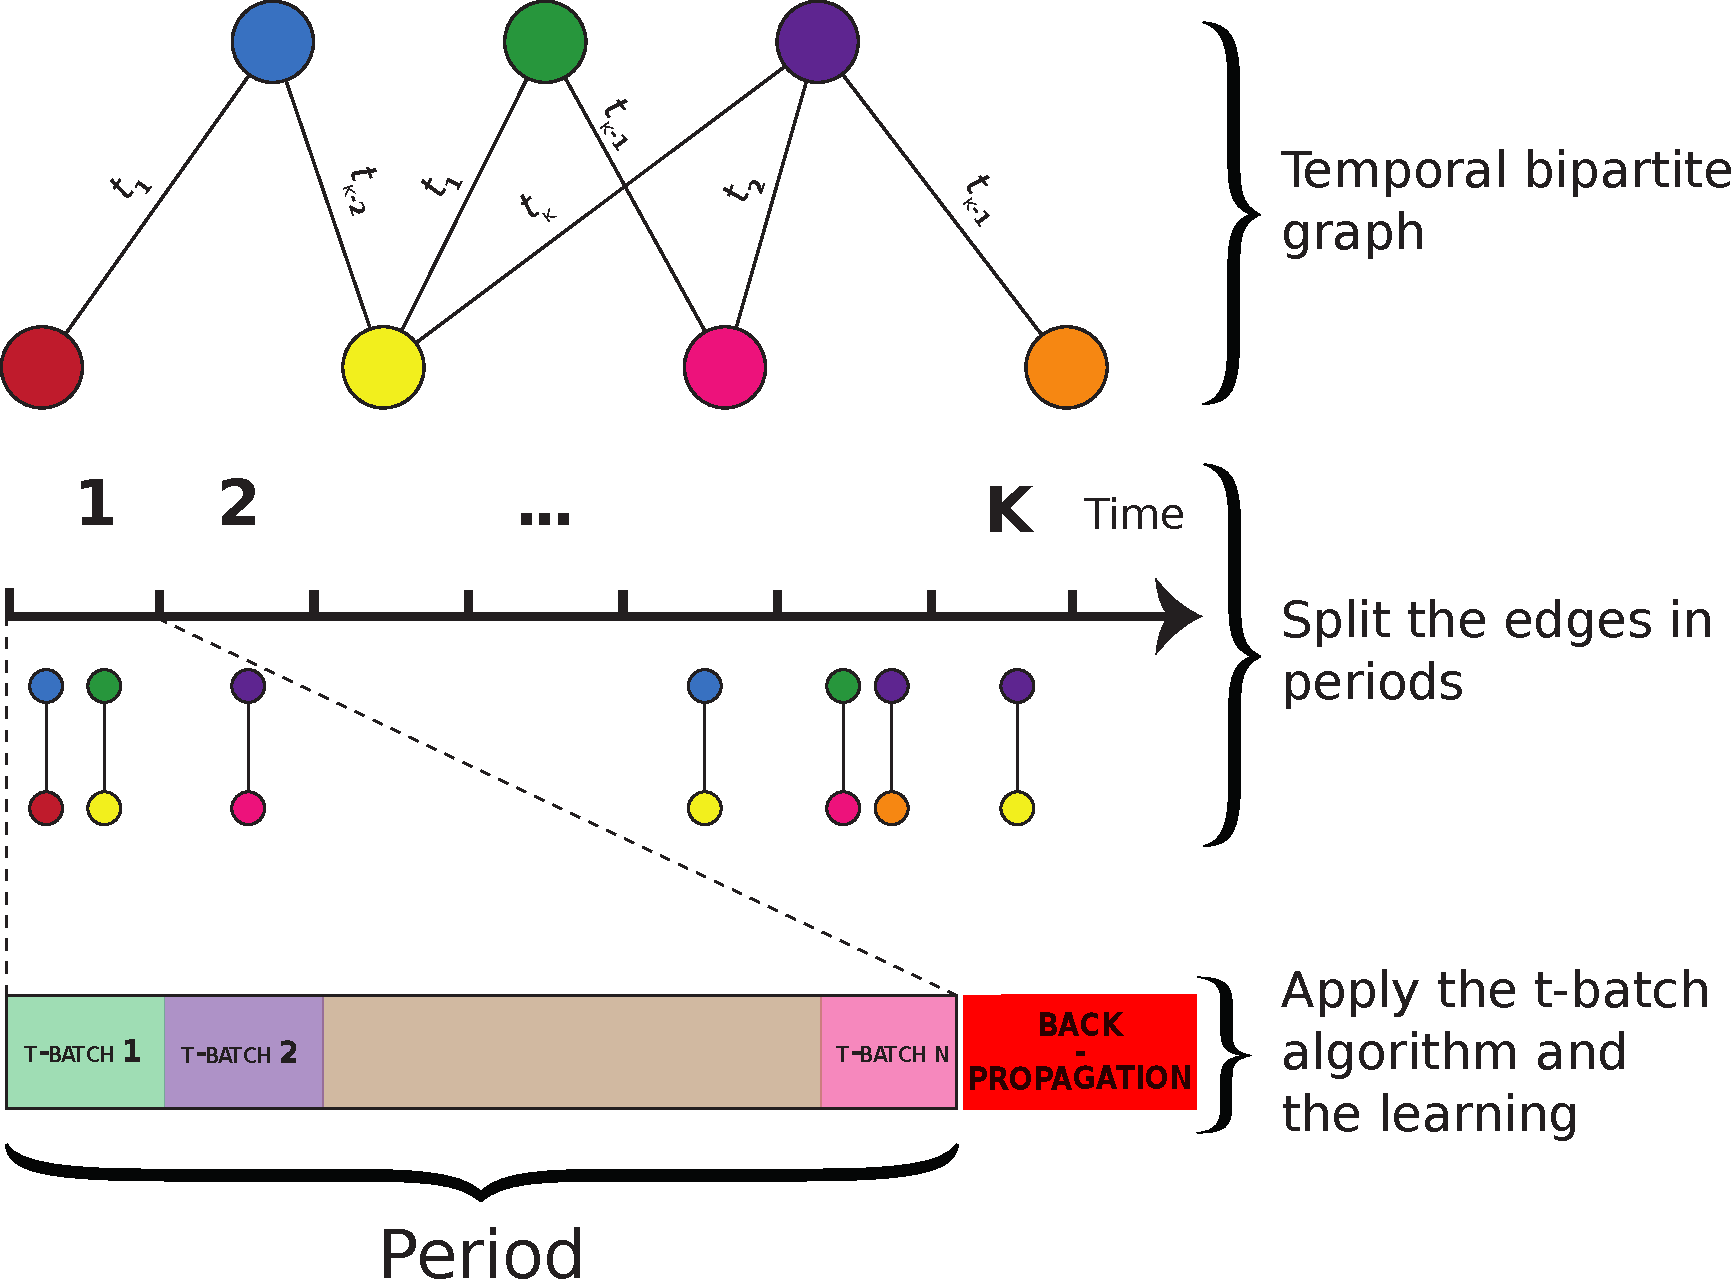
\includegraphics[width=1.0\textwidth]{image/pipeline.pdf}
    \end{center}
    \caption{Pipeline. $MLP_{reg}$ gives an estimation of the embedding of the next item $\textcolor{blue}{\overset{\sim}{i}}$ with which a user $\textcolor{red}{u}$ is likely to interact. The MLP  is designed to recommend the best $\textcolor{blue}{i}$ to each user. $MLP_{classif}$ is used to predict the user's state change $\textcolor{red}{\widehat u_{state}}$. Will the user potentially drop out / get banned ?}
    \label{Pipeline}
\end{figure}

\subsection{Code}
We re-implemented the JODIE model using a newer version of Pytorch~\cite{NEURIPS2019_bdbca288} (version 1.10 and python 3.8 ) independently of the original code provided by the authors\footnote{\url{https://github.com/srijankr/jodie}}.
Our code \and trained models are publicly available at \url{https://github.com/ComplexNetTSP/JODIE.}
We want to point out that we have used the \textit{tanh} function as the activation function at the output of the RNNs (see Figure \ref{Pipeline}) to build our model in accordance with the original code but in contrast to what the authors wrote in the original paper. Our source code is organized as follows:
\begin{itemize}
    \item \textbf{preprocessing.py} includes data preprocessing and the t-batch code.
    \item \textbf{model.py} contains the model as described in Figure \ref{Pipeline}.
    \item \textbf{train.py} is used to train the model.
    \item \textbf{evaluate.py} is used to evaluate the model after the training.
\end{itemize}

Organizing the code this way makes it meaningful and easier to reuse and considerably reduces the effort for code reviews and tests. Before running the model, it is necessary to create an environment with the required packages and run one of the following python scripts to launch the training/evaluation of the JODIE model on one of the available datasets:
\begin{itemize}
    \item \textit{train\_evaluate\_wikipedia.py, train\_evaluate\_lastfm.py, train\_evaluate\_reddit.py}
    \item \textit{train\_evaluate\_reddit\_state.py, train\_evaluate\_wikipedia\_state.py, train\_evaluate\_mooc\_state.py}
\end{itemize}
Further information is available in the GitHub README file.\footnote{\url{https://github.com/ComplexNetTSP/JODIE}}

\subsection{Model description}

\subsubsection{Update operator}
The update operator takes the form of two mutually recursive neural networks as depicted in Figure \ref{recursive RNNs}. RNN$_U$ updates users' dynamic embeddings, whereas RNN$_I$ updates those of the items. The embeddings are thus considered as the hidden states of the classical RNNs. At time $t=0$, the embeddings (noted $u_0$ and $i_0$) are initialized randomly according to a uniform distribution $\mathcal{U}[0;1[$ followed by a normalization. In addition to the embeddings at time $t=0$, the RNNs take as input $\Delta$, the time elapsed between an entity and the previous interaction, and $f$ a feature vector which characterizes the link of the interaction. As we can observe, the specificity of these RNNs is that they take four inputs instead of the standard two. In order to narrow down to just two entries, the embeddings of the other entity $\Delta$ and $f$ are concatenated. In Figure \ref{recursive RNNs}, $[.,.]$ is used to denote the concatenation. More formally, the embeddings are updated with the following formulas:

$$
u^+ = \sigma \left ( W_1^u u^- + W_2^u i^- + W_3^u f + W_4^u \Delta_u \right )
$$
$$
i^+ = \sigma \left ( W_1^i i^- + W_2^i u^- + W_3^i f + W_4^i \Delta_i \right )
$$

where the matrices $W_1^e, ..., W_4^e$ are the parameters of the RNN$_e$\textcolor{green}{?} and $\sigma$ an activation function (here hyperbolic tangent). $u^-$ and $i^-$ represent the embeddings before updating and $u^+$ and $i^+$ represent the embeddings after updating. Once this step is finished, the next operation, called the projection operation, can be launched.

\begin{figure}[htbp]
   \centering
    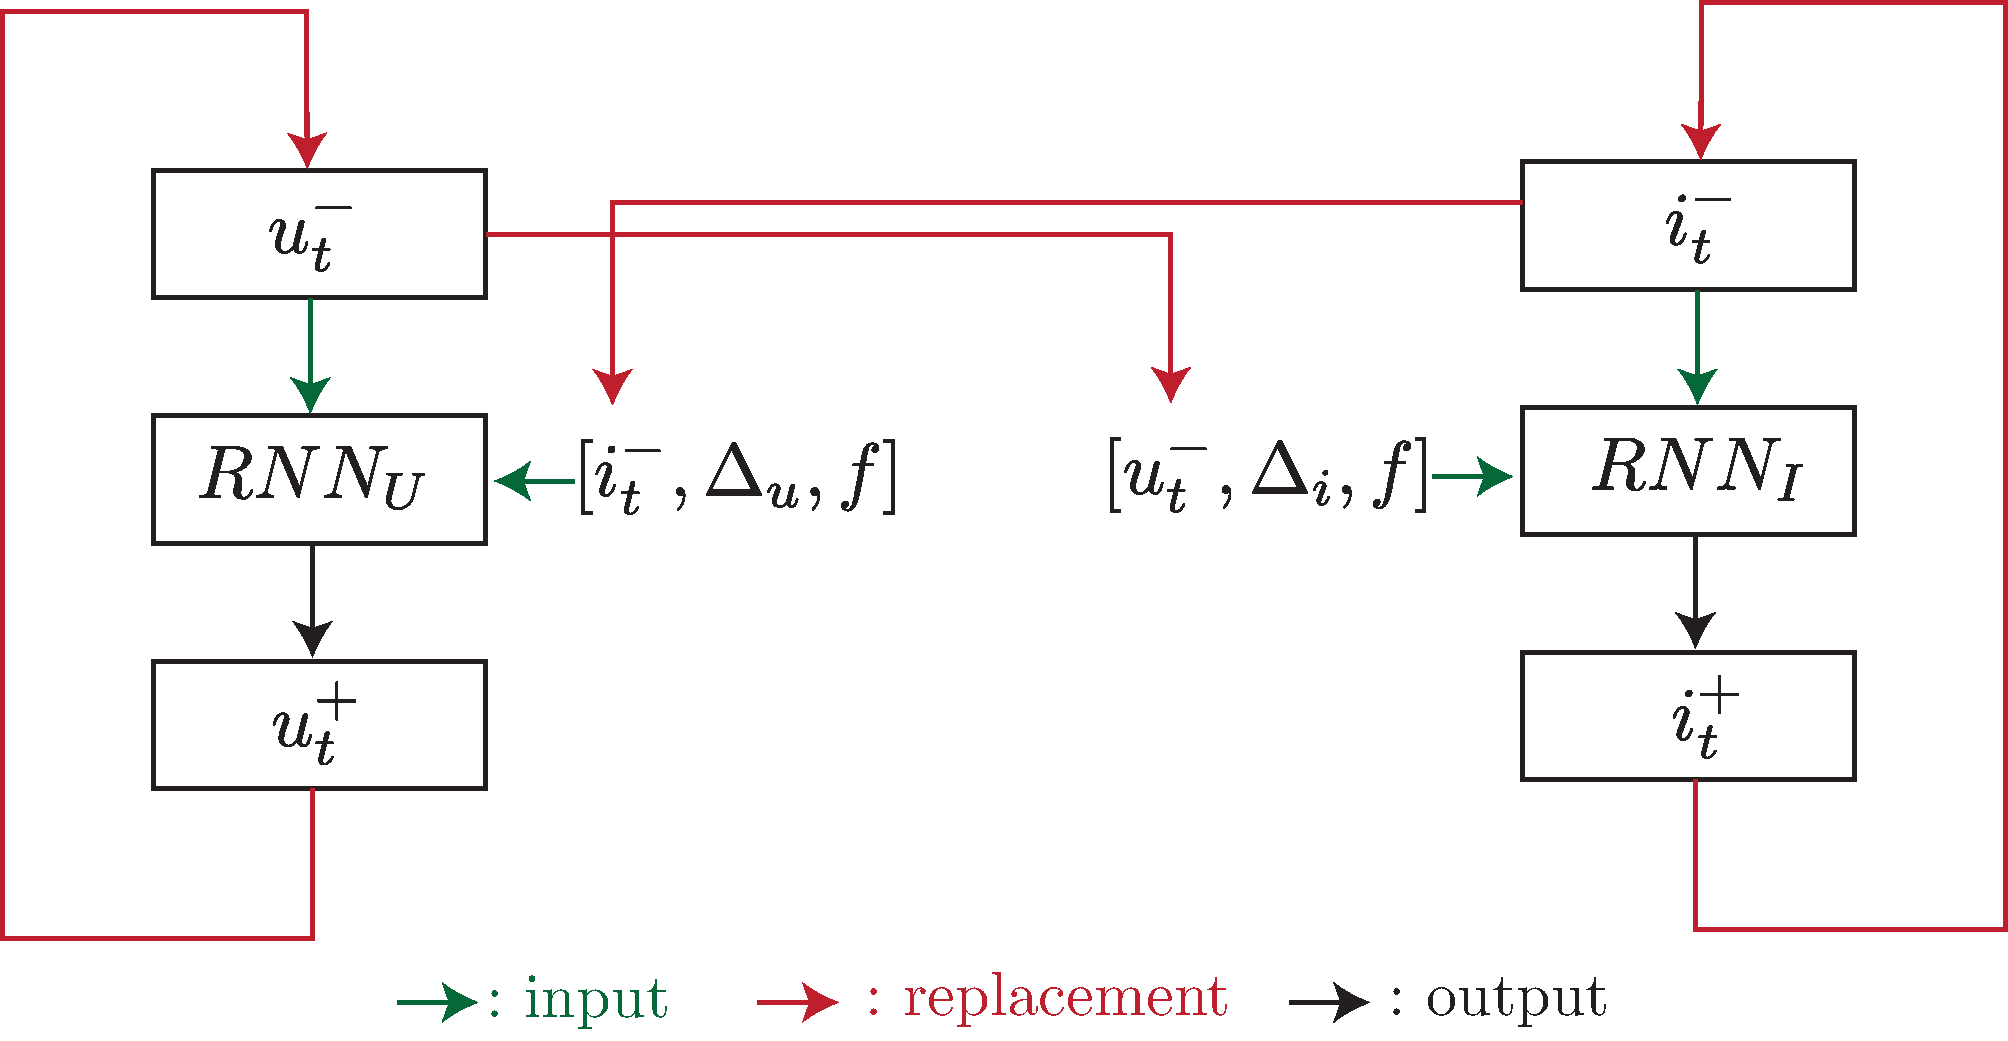
\includegraphics[width=1.0\textwidth]{image/rnn_jodie.pdf}
    \caption{RNN mutually recursive \textcolor{green}{[1]}}
    \label{recursive RNNs}
\end{figure}

\subsubsection{Projection operation}

This operation consists in projecting the user's embeddings to a future time. Indeed, as users' interests evolve over time, modeling this variation as a linear projection is particularly appropriate. For a deeper understanding, please refer to the original figure provided by the authors in Figure~\ref{recursive RNNs}. We notice that over a very short time interval, the projected embedding of the user changes slightly, but as time goes by, the projected embedding will be further away from its original embedding. To perform this operation, $\Delta$ is converted into a vector $w \in \mathbb{R}^n$ using a linear layer represented by its weights vector $W_p$. We have $w = W_p \Delta$.  We initialize $W_p$ by a Gaussian of zero mean. We obtain the projected embedding by computing the Hadamard product, denoted $*$, of $1+w$ and $u_t$. The authors use the following formula.

$$
\widehat u_{t+\Delta} = (1+w) * u_t
$$

We can see that if $\Delta = 0$, then $w=0$ and the projected embedding is the same as the initial embedding. We can consider this operation as a simple linear transformation. Both operators are used to learn the model. One limitation cited by the authors is the learning time. Indeed, the existing models process each interaction one after the other, which takes a considerable amount of time. The authors have proposed an algorithm called \texttt{t-batch}, that splitsctemporal data into batches, which considerably speeds up the learning time.

\subsubsection{t-Batch algorithm}

%The 
%\texttt{t-Batch} %algorithm 
it is a linear algorithm, %that
\textcolor{green}{and its general idea is to split} temporal data into batches 
(see Figure~\ref{pipeline_t-batch}).However, it is not easy to figure out the details of its functionality simply after reading the article or studying the source code. Indeed, the original paper presents the algorithm in only a few sentences. Moreover, the code is embedded with other pieces of code in the learning loop, making it challenging to grasp its behavior.To shed light on this algorithm which is the cornerstone of the authors' contribution, we propose the algorithm \ref{t-batch}. It takes as input a list of time-stamped events and distributes them in a batch according to the following two constraints: first, it ensures that the same batch cannot contain the same entity several times. Secondly, it ensures that temporal dependencies within and between batches are preserved. In other words, the interactions are processed in sequence. These two requirements guarantee that the batches are independent (and parallelizable). The computation of the batch index, $B_{idx}$, in which the interaction $\mathcal{S}_r \in \mathcal{S}$ will be placed, is done in line 9 of the algorithm. 

\begin{algorithm}[htbp]
    \caption{t-Batch}
    \label{t-batch}
    \begin{algorithmic}[1]
        \STATE \textbf{Input} : Sequence of interactions ordered by time $S$ : $S_j = (u_j,\,i_j,\,t_j,\,f_j)$
        \STATE \textbf{Output} : Sequence of batches $B$ : $B_k = \{S_{k,1},\,...,\,S_{k,n} \}$
        \STATE \textbf{Initialize} : 
        \STATE \quad $\text{tbatch\_id\_u[u]} \leftarrow 0 \; \forall \; u \in \mathcal{U}$, \quad $\text{tbatch\_id\_i[i]} \leftarrow 0 \; \forall \; i \in \mathcal{I}$
        \STATE \quad $B_k \leftarrow \{ \},\; \forall \; k \in$ [\![$1,\;\text{Card}(S)$]\!]
        \STATE \quad $C \leftarrow 0$
        \FOR{$S_j \in S$}
            \STATE $(u_j,\,i_j,\,t_j,\,f_j) \leftarrow S_j$
            \STATE idx $\leftarrow$ $\max$(tbatch\_id\_u[$u_j$], tbatch\_id\_i[$i_j$]) + 1
            \STATE $B_\text{idx} \leftarrow B_\text{idx} \cup \{ S_j \}$
            \STATE tbatch\_id\_u[$u_j$] = idx
            \STATE tbatch\_id\_i[$i_j$] = idx
            \STATE $C \leftarrow \max(C,\,$idx)
        \ENDFOR
        \RETURN $\{ B_1,\,...,\,B_C \}$
    \end{algorithmic}
\end{algorithm}

\subsubsection{Next item embedding and state change losses}

The JODIE model has been designed to give directly an embedding of an item, which is time saving. Indeed, the existing models predict a probability for each item. This can be very long if the dataset contains many items. JODIE will produce an embedding and the suggested item will be the one whose embedding will be the closest to the one of the prediction. 
\textcolor{green}{The JODIE model has been designed to produce an item embedding, representing significant time-saving. As a matter of fact, the existing models predict a probability for each item, which might be time-consuming for large datasets. So instead, JODIE produces an embedding, and the suggested item is the one whose embedding is the closest to the one of the prediction. }

To make this prediction, \textcolor{green}{a neural network takes as input} %we use a neural network that will have as input 
the projected embedding of the user at time $t+\Delta$ noted $\widehat u(t+\Delta)$ and the embedding of the previous item of the user before time $t+\Delta$ noted $i(t+\Delta^-)$. This embedding is important because  \textcolor{green}{an} item can interact with other users between time $t$ and $t+\Delta$, which means that it contains more recent information. JODIE uses both static and dynamic embeddings, denoted respectively $\Bar{e}$ and $e$, to make the prediction of a static and dynamic embedding $\overset{\sim}{i}$. The prediction is done with a fully connected linear layer.
$$
\overset{\sim}{i} (t+\Delta) = W_1 \widehat u(t+\Delta) + W_2 \Bar{u} + W_3 i(t+\Delta^-) + W_4 \Bar{i} + B
$$
Where $W_1, ..., W_4$ and the bias vector $B$ are the model weights.\\

JODIE is trained to minimize the L2 distance between the predicted embedding and the real item embedding of each interaction. %We compute the 
\textcolor{green}{The} loss function \textcolor{green}{is computed} as follows:

\begin{equation}
    \textit{Loss} = \sum_{(u,\,i,\,t,\,f) \in S} \| \overset{\sim}{i}_t - [\Bar{i},\,i_t^-] \|_2 + \lambda_U \|u_t - u_t^-\|_2 + \lambda_I \|i_t - i_t^-\|_2
\end{equation}

The first term minimizes the error of the predicted embedding. The next two terms regulate the loss function, and ensure that  
the dynamic embeddings of users and items do not vary too much. $\lambda_U$ and $\lambda_I$ are the regularization terms that penalize the two terms. In the original paper, the authors fixed the values of $\lambda_U$ and $\lambda_I$ as $\lambda_U = \lambda_I = 1$, without much justification. But it is unclear whether this is the best value or if another value would be more appropriate. 

When we want to predict the change of state of a user, we use the same loss function with an additional term which is the cross-entropy. To do this, we have to make sure that the classes are binary. In this case, it is possible to train the model using an additional loss term function that will make it able to predict the labels using the user's embedding after an interaction. The additional loss function term, for predicting a user's state change, is a weighted cross-entropy expressed in the following equation:

When it comes to predicting the change of state of a user, we use the same loss function with an additional term, cross-entropy. To do so, we need to guarantee that the classes are binary. In this case, it is possible to train the model using an additional loss function that makes it capable of predicting labels utilizing the user's embedding after an interaction. The loss function  term for predicting a user's state change is a weighted cross-entropy expressed in the following equation:

\begin{equation}
    \ell(x,y) = \sum_{n=1}^N \frac{l_n}{\sum_{n=1}^N w_{y_n}} \; \text{ with } \;
    l_n = -w_{y_n} \log \left ( \frac{\exp(x_{n,y_n})}{\sum_{c=1}^C \exp(x_{n,c})} \right )
\end{equation}

Where $x$ is the input, $y$ is the target, $w$ is the weight, $C$ is the number of classes (here two) and $N$ is the batch size. The loss function becomes:

\begin{equation}
    \textit{Loss} = \sum_{(u,\,i,\,t,\,f) \in S} \| \overset{\sim}{i}_t - [\Bar{i},\,i_t^-] \|_2 + \lambda_U \|u_t - u_t^-\|_2 + \lambda_I \|i_t - i_t^-\|_2 + \ell (u_{true}, \widehat u_{pred})
\end{equation}

Where $u_{true}$ is the real class of the user and $\widehat u_{pred}$ his predicted class. It is also worth noting that the %regularizations 
regularization terms are MSE. The authors wanted the embeddings not to vary heavily between the previous time $t-1$ and the current time $t$. Indeed, they started from the postulate that the behavior of a user represented by its dynamic embedding does not vary considerably over a small temporal interval.\\

\subsubsection{Training JODIE model} 
\label{sec:trainning}

We detail \textcolor{green}{here} the learning steps and the code simplification of JODIE model we provide like the use of functions (steps 1, 3-7) or the t-bach computation?? (in step 3). 
\begin{enumerate}
    \item We use a function called \textbf{preprocess} which is in the file \textbf{preprocessing.py} to make a pre-processing of the data to extract information necessary during the training. Information like the sequence of users, items, time, features, or previous items that will be used during the learning step.
    \item We initialize each embedding randomly $\mathcal{U}([0,1[)$.
    \item During the training phase, the observations are usually split from the original dataset into a given number of batches (K times periods, see Figure \ref{pipeline_t-batch} for more details). To overcome this issue, JODIE uniformly splits the data into ordered batches, and then, the \texttt{t-batch} algorithm is applied independently on each subset of the data as described in Figure \ref{pipeline_t-batch}.  It is worth noting that our implementation of the t-batch algorithm differs from what was originally defined in \cite{kumar18}. Instead of applying the \texttt{t-batch} function at each run, we perform all the t-batches in a single run with the  function \textbf{t\_batch} in the \textbf{preprocessing.py} file before the learning step, looping over the periods.
    \item During the learning stage, in the function \textbf{train\_ray} in the file \textbf{train.py}, we use the function \textbf{projection} from the file \textbf{model.py} to project users' embedding in a future time. We also use the function \textbf{predict\_embedding\_item} in the file \textbf{model.py} to make a prediction of the next embedding of the item. And finally, we calculate the Mean Square Error (MSE) of the predicted embedding and the real embedding.
    \item We update embeddings of users and items using the functions \textbf{update\_rnn\_user} and \textbf{update\_rnn\_item} respectively in the file \textbf{model.py}.
    \item We compute the two regularization terms using the function \textbf{regularizer} of the file \textbf{preprocessing.py}. This function uses the hyperparameter $\lambda_e$.
    \item If necessary, we predict the state prediction and we calculate the loss Cross Entropy (CE) with the function \textbf{loss\_predict\_state} of the file \textbf{model.py} which makes the prediction and the calculation of the loss.
    \item We perform the back propagation of the gradient, at the end of a period, to update the model weights.
    \item Once all the time periods are covered, we go to the next epoch.
\end{enumerate}
Once the learning stage is over, the evaluation is carried out.

\begin{figure}[htbp]
    \centering
    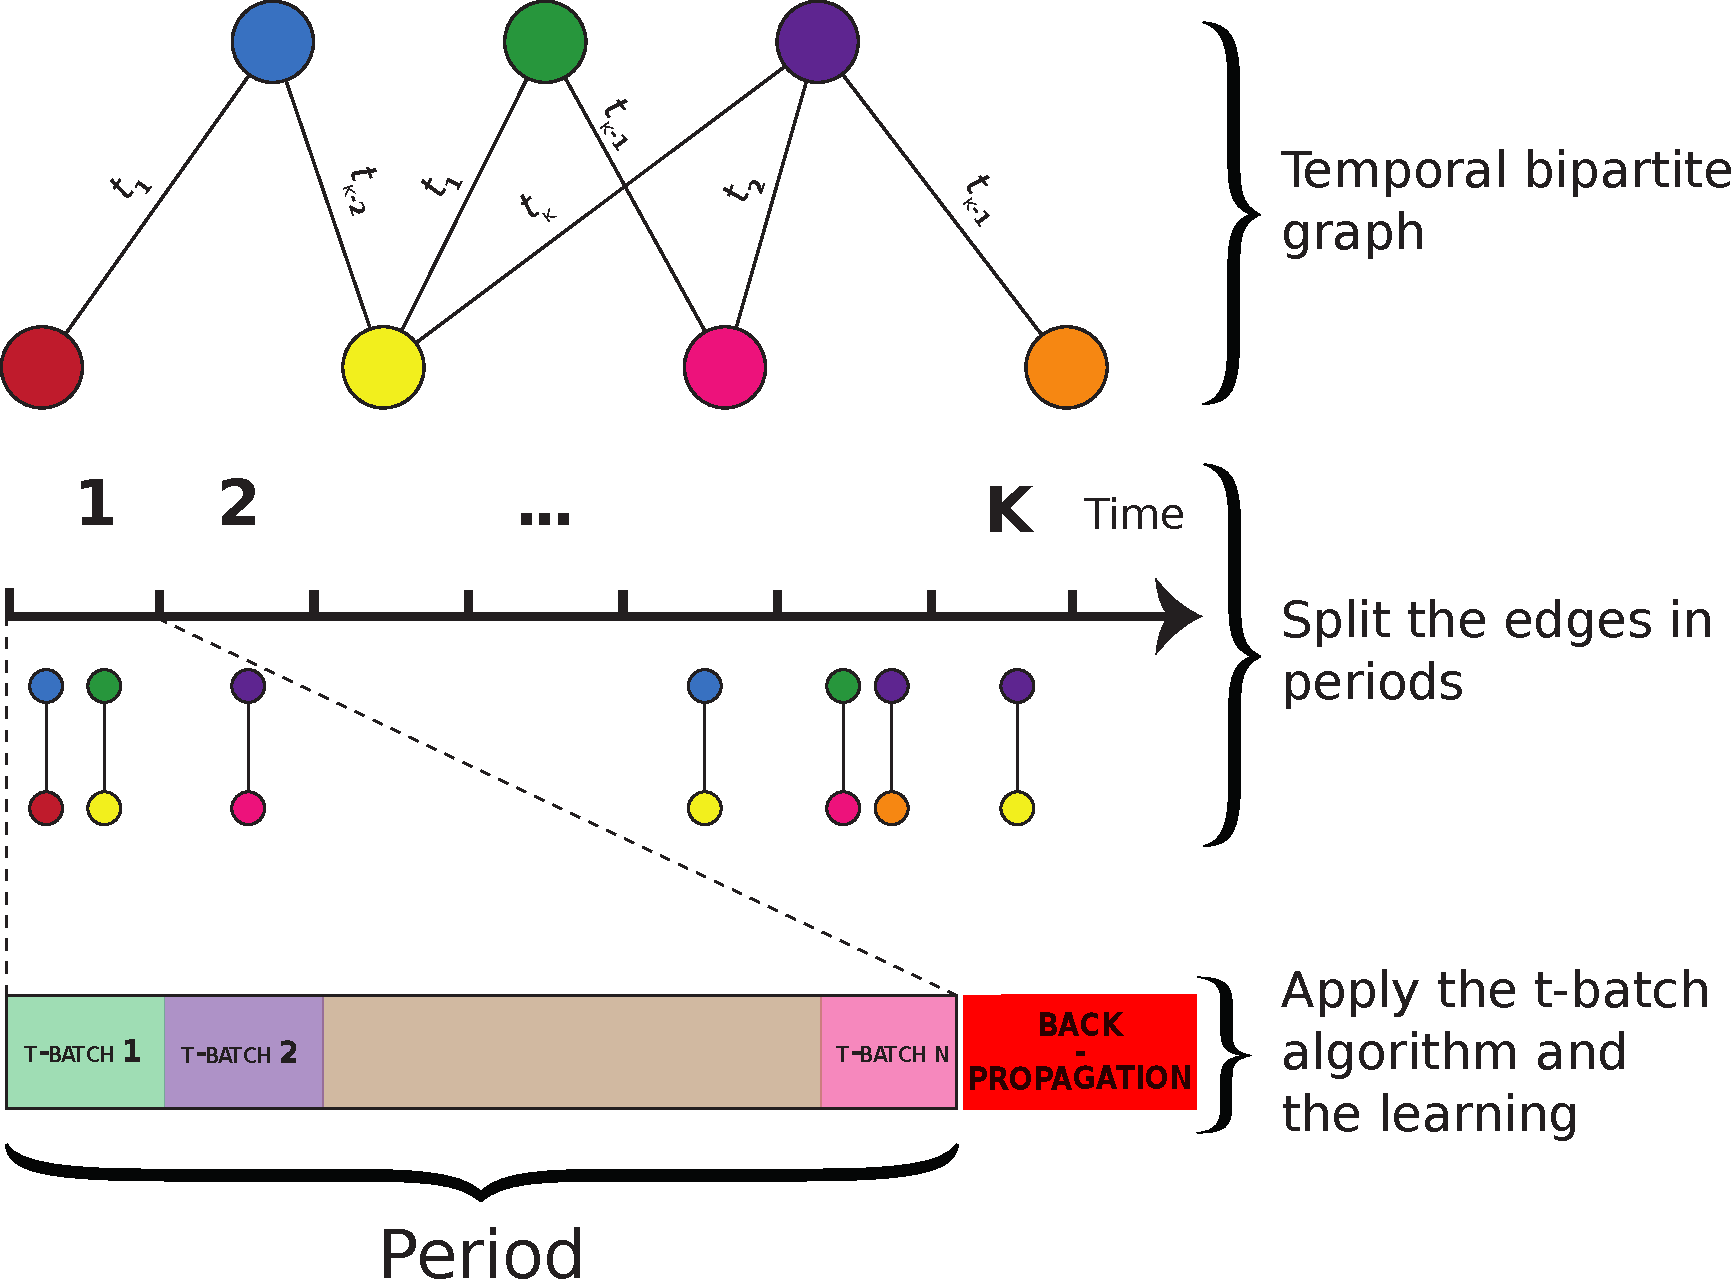
\includegraphics[width=.7\textwidth]{image/pipeline_t-batch.pdf}
    \caption{Pipeline of the \texttt{t-batch} algorithm}
    \label{pipeline_t-batch}
\end{figure}

\subsubsection{Prediction and evaluation JODIE model}
During the prediction task as oppose to the trainning task we will  process the interactions one at the time. The prediction task is share the step 4-8 with the trainning task. Depending of which prediction task we want to perform (either predict a state change or predict the next item embedding), we will use either the \textbf{predict\_state} function in the \textbf{model.py} file or the \textbf{predict\_embedding\_item} function in the \textbf{model.py} file.

\subsection{Datasets}
 
The data sets that were used in the original article were also used in this work. The authors of the article give the datasets. \\

\textcolor{green}{We used the datasets provided by the authors, but we had to pre-process them as the format was not directly usable.} \\

\textbf{Reddit~\cite{Reddit} post dataset}: this public dataset consists of one month of \textcolor{green}{user posts} %posts made by users 
on subreddits. We selected the 1000 most active subreddits as items and the 10000 most active users. We convert the text of each post into a feature vector representing their Linguistic Inquiry and \textcolor{green}{Word} %Work 
Count~\cite{pennebaker01LIWC} (LIWC) categories.\\
\textbf{Wikipedia~\cite{Wiki} edits}: this public dataset is one month of edits made by edits on Wikipedia pages. We selected the 1000 most edited pages as items and editors who made at least 5 edits as users (a total of 8227 users). Similar to the Reddit dataset, we convert the edit text into a LIWC feature vector.\\
\textbf{LastFM~\cite{10.1007/978-3-642-33486-3_5lastFM} song listens}: this public dataset has one month of who-listens-to-which song information. We selected all 1000 users and the 1000 most listened songs. In the dataset, interactions do not have features.\\
\textbf{Reddit bans}: Reddit post dataset with ground-truth labels of banned users from Reddit. This gives 366 true labels (=0.05\%).\\
\textbf{Wikipedia bans}: Wikipedia edit data with public ground-truth labels of banned users. This results in 217 positive labels (=0.14\%).\\
\textbf{MOOC~\cite{mooc} student drop-out}: this public dataset consists of actions done by students on a MOOC online course. This dataset consists of 7047 users interacting with 98 items. There are 4066 drop-out events (=0.98\%). All datasets and their details are shown in Table \ref{description data}. \\

\setlength\tabcolsep{0.12cm} % changer l'écart entre les colonnes pour faire rentrer sur la bonne largeur.
\begin{table}[htbp]
    \centering
    \ra{1.3}
    \begin{tabular}{@{}lrrrrcc@{}}
    \toprule
    & Users & Items & Interactions & State changes & Action repetition & Features size \\
    \midrule
    Reddit & 10,000 & 984 & 672,447 & 366 & 79\% & 172 \\
    Wikipedia & 8,227 & 1,000 & 157,474 & 217 & 61\% & 172 \\
    LastFM & 980 & 1,000 & 1,293,103 & -\textcolor{white}{0} & 8.6\% & 2 \\
    MOOC & 7,047 & 97 & 411,749 & 4,066 & - & 4 \\
    \bottomrule
    \end{tabular}
    \caption{Description of the datasets that were used in this project}
    \label{description data}
\end{table}
\setlength\tabcolsep{6pt} 

The authors of the original paper created their own datasets. Thus, a dataset has the following format :
\begin{itemize}
    \item A line represents an interaction or an edge
    \item Each line is described by a user, an item, a timestamp, a state label, and features
    \item The timestamp is in cardinal number format
    \item The state label is \textcolor{green}{equal to} 1 if the user changes \textcolor{green}{his} state and 0 otherwise. If there are no state labels, use 0 for all interactions
    \item Features can be as long as desired and of dimension at least \textcolor{green}{equal to} 1. If there is no feature, use 0 for all interaction\textcolor{green}{s}
\end{itemize}
A negative point about the data sets is that the variable names are not in the right places and this creates errors when using them. That is why we created a function called \textbf{fetch\_datasets} in the file \textbf{preprocessing.py} which allows to have correct variable names which have the following format: 
\textcolor{green}{
A negative point regarding the datasets is that the variable names are not in the right place, causing errors when using them. To fix this issue, we came up with a function called \textbf{fetch\_datasets}(available in the \textbf{preprocessing.py} file) that produces correct variable names in the following format:}

\texttt{user, item, timestamp, labels, f\_1, ..., f\_$n$} with $n$ the number of features.\\

\subsection{Hyperparameters}

As described in the model descriptions section, the model has several hyperparameters like epoch number, dynamic embedding size, learning rate, \texttt{split}, $\lambda_U$ and $\lambda_I$. Initially, the hyperparameters were chosen as in the original article as follow\textcolor{green}{s}.

\begin{itemize}
    \item Embedding size: $32, \, 64, \, \textbf{128}, \, 256$
    \item Epoch, learning rate, $\lambda_U$ and $\lambda_I$: $50, \, 10^{-3}, \, 1, \, 1$ respectively
    \item \texttt{Split}: $500$
\end{itemize}

\textcolor{green}{In the original paper, }only the size of the dynamic embeddings \textcolor{green}{has} %have 
been studied and chosen using a grid search. The other hyperparameters are just given without any justification.

\subsection{Extended experiments}


Of all these hyper-parameters, the one that caught our eye the most was \texttt{split}. Indeed, \texttt{split} is used to define the frequency at which t-batches are created and the JODIE model is trained. It is important to choose its value well to have enough data in a period. 

\textcolor{green}{Among all these hyperparameters, the one that caught our attention the most is \texttt{split}. Indeed, \texttt{split} defines the frequency at which the t-batches are generated, and the JODIE model is trained. Therefore, it is crucial to carefully choose its value to ensure sufficient data in a period. }

To test this hyper-parameter, we set the other hyper-parameters \textcolor{green}{as follows: }%to 
$50$ epoch, $\lambda_U = \lambda_I = 1$, learning rate = $1e-3$, and the size of the embeddings to $128$. \textcolor{green}{We then assign the following values to \texttt{split}: $5$, $500$ and $50000$}

%, and we test these $5$, $500$ and $50000$ for the value of \texttt{split}. 
%We define \texttt{split} as follows:
%\texttt{split} is used to split the dataset for a specific period of time\textcolor{green}{???}. 


%The authors use it as follows : $\frac{\text{time}_{\text{end}} - \text{time}_{\text{start}}}{\text{\texttt{split}}}$\textcolor{green}{???}. 

\section{\textcolor{green}{Computational requirements}}
\textcolor{green}{The experiments were reproduced on ... ?cores ? RAM ...? processor...}



\section{Results}
\textcolor{green}{In this section, we will discuss the results of the conducted experiments}
%In this section, we will present the results obtained with replication. 
%First, we tried to replicate the results for the user's state change prediction on all available datasets. The strategy  was to predict only with the model weights obtained in the last learning epoch while the authors decided to keep the best epochs weights. For this prediction task, other embedding sizes were tested like 8, 16 and 32. Then, we tried to reproduce the results for the future interaction prediction using the same strategy as for the state prediction. Then a second part was devoted to adding results that are not present in the original paper like the importance of the \texttt{split} hyper-parameter.
\textcolor{green}{First, we replicated the results of predicting the user's state change over all available datasets. Our strategy was to predict only with the model weights obtained in the last training epoch, whereas the authors kept only the best epoch weights. In addition, we tested other integration sizes for this prediction task, such as 8, 16, and 32. Then, we replicated the results for future interaction prediction using the same strategy. Finally, after reproducing the results, we added some results that were not provided in the original paper, such as the importance of the hyperparameter \texttt{split}.}

\subsection{Core replication results}
The first part of the results concerns the prediction of the user's state change. The model has for hyperparameters a \texttt{split} of $500$, $\lambda_U = \lambda_I = 1$ as those in the original paper and the embedding size varies. We present the results obtained for embeddings of size $32$, $128$ and $256$ as well as the results of the original paper in the Table~\ref{result-state}.

\begin{table}[htbp]
    \centering
    \ra{1.3}
    \begin{tabular}{@{}lcrrrr@{}}
    \toprule
    & JODIE & \phantom{abc} & \multicolumn{3}{c}{Replications} \\
    \cmidrule{2-2} \cmidrule{4-6}
    & 128 && \multicolumn{1}{c}{32} & \multicolumn{1}{c}{128} & \multicolumn{1}{c}{256} \\
    \midrule
    Reddit & $\boldsymbol{0.599}$ && $0.563 \pm 0.013$ & $0.586 \pm 0.018$ & $0.577 \pm 0.012$\\
    Wikipedia &$\boldsymbol{0.831}$ && $0.728 \pm 0.010$ & $0.738 \pm 0.030$ & $0.711 \pm 0.008$\\
    MOOC &$\boldsymbol{0.756}$ && $0.688 \pm 0.006$ & $0.718 \pm 0.021$ & $0.711 \pm 0.004$\\
    \bottomrule
    \end{tabular}
    \caption{Results: user state change prediction}
    \label{result-state}
\end{table}

We observe, for the Reddit dataset, a performance of $0.586$ AUC for the reproduction against $0.599$ in the original paper. We also notice a  $0.718$ AUC  for the MOOC dataset results, which is close to the $0.756$ AUC obtained in the original paper. For Wikipedia dataset, we can observe a performance of $0.738$ AUC for the reproduction and $0.831$ AUC for the original model. On the Reddit, Wikipedia, and MOOC datasets, we see a standard deviation of $0.018$, $0.030$, and $0.021$, respectively for an embedding size of 128. We can explain this difference by the fact that the authors of JODIE evaluated their models on each epoch and chose the best performance in \textcolor{green}{the} validation while our results come from the \textcolor{green}{fiftieth} %50 
and last epoch. This can explain the difference between their results and \textcolor{green}{ours,} %our results 
but this difference remains nevertheless marginal.

%We can see that if we increase the size of the embeddings to 256, the results degrade slightly. This can be due to size of the embeddings which is too big which allows fitting some noise from the data. Conversely, if the size of the embeddings is 32, the results are worse. This can be explained by the fact that the embeddings are too small and lack information to make a good prediction.\\

\textcolor{green}{We can observe that if we increase the size of the embeddings to 256, the results degrade slightly. This may be caused by the embedding size being too large, thus including some noise in the data. Conversely, if the embedding size is 32, the results are worse. This can be explained by the fact that the embeddings are too small and lack information to make a good prediction.}

For the prediction of future interaction, we used the same hyperparameters as for the state prediction. We present the obtained results and the results of the original paper in Table~\ref{result-interaction}.

\begin{table}[htbp]
    \centering
    \ra{1.3}
    \begin{tabular}{@{}lccccc@{}}
    \toprule
    Dataset\hspace*{3em} & JODIE & \phantom{abc} & \multicolumn{3}{c}{Replications} \\
    \cmidrule{2-2} \cmidrule{4-6}
    & 128 && \multicolumn{1}{c}{32} & \multicolumn{1}{c}{128} & \multicolumn{1}{c}{256} \\
    \midrule
    \multicolumn{1}{l}{\hspace{-0.2cm}\textbf{Reddit}} \\
    {\quad \small MRR} & $\boldsymbol{0.726}$  && $0.711 \pm 0.007$ & $0.719 \pm 0.008$ & $0.684 \pm 0.005$ \\
    {\quad\small Recall@10}  &$\boldsymbol{0.852}$ && $0.810 \pm 0.020$ & $0.830 \pm 0.020$ & $0.747 \pm 0.011$\\
    \multicolumn{1}{l}{\hspace{-0.2cm}\textbf{Wikipedia}}\\
    {\quad\small MRR} &$0.746$ && $\boldsymbol{0.763} \pm 0.005$ & $\boldsymbol{0.764} \pm 0.002$ & $\boldsymbol{0.763} \pm 0.004$  \\
    {\quad\small Recall@10}  & $0.822$ && $\boldsymbol{0.829} \pm 0.005$ & $\boldsymbol{0.833} \pm 0.004$ & $\boldsymbol{0.827} \pm 0.004$\\
    \multicolumn{1}{l}{\hspace{-0.2cm}\textbf{LastFM}} \\
    {\quad\small MRR} &$0.195$ && $\boldsymbol{0.311} \pm 0.001$ & $\boldsymbol{0.313} \pm 0.002$ & $\boldsymbol{0.312} \pm 0.001$ \\
    {\quad\small Recall@10}  & $0.307$ && $\boldsymbol{0.455} \pm 0.003$ & $\boldsymbol{0.483} \pm 0.047$ & $\boldsymbol{0.453} \pm 0.002$\\
    \bottomrule
    \end{tabular}
    \caption{Results: future interaction prediction}
    \label{result-interaction}
\end{table}

We notice that only the results on the Reddit dataset are slightly lower than in the original paper. On these data, we obtained 0.719 in MRR and 0.830 in Recall@10. However, these results remain close to those obtained by the authors with 0.726 in MRR and 0.852 in Recall@10. For the Wikipedia and LastFM datasets, we can see that our results outperformed the authors' results with 0.764 in MRR and 0.833 in Recall@10 and 0.313 in MRR and 0.483 in Recall@10 respectively. These differences can be explained by the choice to evaluate the last epoch and not to choose the best performance on the validation, nonetheless these differences remain small.\\

To go further in the replication and reproduction, we  will also reproduce two figures that show that the robustness of JODIE model (see Figure~\ref{percentage-train})\textcolor{green}{????}. 


\textcolor{green}{To go further in the replication and reproduction, we plot in Figure ~\ref{percentage-train} the performances of JODIE for both state change and  interaction prediction (Figure ~\ref{percentage-train} B) tasks on Wikipedia dataset. \\
For state change prediction  (Figure ~\ref{percentage-train}  A), we varied the percentage of the training set from 20\% to 60\% in 10\% steps. The results show that the larger the training is, the less the model is accurate in predicting state change due to class imbalances.  }
%The Figure~\ref{percentage-train} A) will be on the same dataset but for the prediction of user state change. 
%For this, we varied the percentage of the training set from 20\% to 60\% in 10\% steps. For the state changes prediction in Figure \ref{percentage-train} A) shows that due to class imbalances, the larger the training is, less the model is accurate in predicting state change. 

\begin{figure}[htbp]
    \centering
    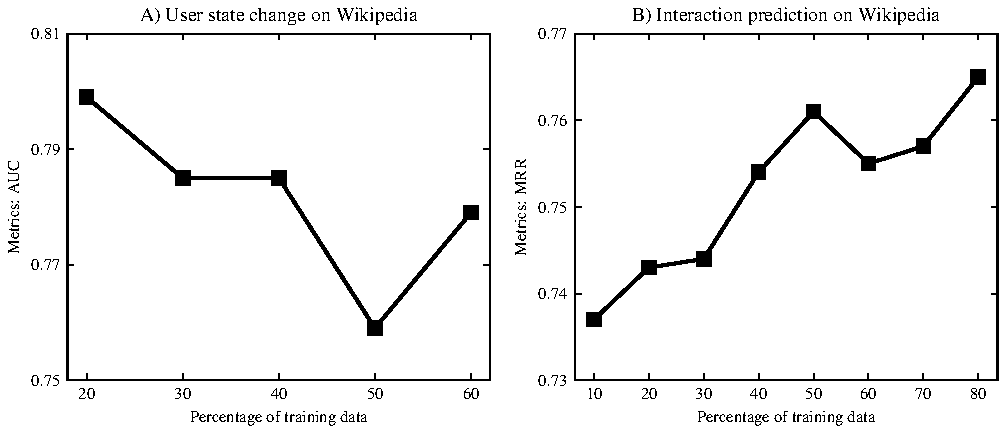
\includegraphics[width = \textwidth]{image/percentage_train.pdf}
    \caption{Robustness of JODIE replication: Figure A) shows the AUC of user state change prediction task by varying the training data size.  Figure B) compares the MRR of JODIE replication with \textcolor{red}{baselines} on interaction prediction task, by varying the training data size. }
    \label{percentage-train}
\end{figure}

\textcolor{green}{Figure ~\ref{percentage-train} B) plots the change in mean
reciprocal rank (MRR) as the training data size is increased. We varied the percentage of the training set from 10\% to 80\% with 10\% step. Contrary to the state change prediction, the larger the training set is, the better the model can predict the future interactions. This behavior is rather typical, where more training data leads to better results (a similar observation was made in the original paper). }
%The Figure~\ref{percentage-train} B) will concern the prediction of future interaction on the Wikipedia dataset by plotting the MRR. For this figure, we varied the percentage of the training set from 10\% to 80\% with 10\% step. 
%On the contrary with the interaction prediction as shown in the Figure \ref{percentage-train} B), larger the training set is, the better is the model will be able to predicting the future interactions. This describes the classical behavior, where the more training data will lead to better results (similar observation was made in the original paper).

%Additionally, we tested the impact of the embedding size on the model. In Figure \ref{emb-size} A)  shows the MRR results of predicting future interactions for the datasets LastFM and Wikipedia and in the Figure \ref{emb-size} B), we show the same results but with the recall@10. Despite the authors claim that the overall performance doesn't depend on the embedding size, in Figure \ref{emb-size},  we show that depending on the metric of interest (i.e.: MRR or Recall@10) the embedding size has an impact on the overall performance of the model. 

\textcolor{green}{Additionally, we tested the impact of the embedding size on the model. Figure \ref{emb-size} A)  shows the MRR results of predicting future interactions for the  LastFM and Wikipedia datasets, and  Figure \ref{emb-size} B) plots the same results but with the recall@10. Although the authors claim that the overall performance doesn't depend on the embedding size, in Figure \ref{emb-size},  we show that depending on the metric of interest (i.e.: MRR or Recall@10) the embedding size has an impact on the overall performance of the model. }

%As conclusion, after having reproduced their results we also claim that their model outperforms the existing models on these 4 datasets and that the replication and reproduction are validated.

\textcolor{green}{As a conclusion, after having reproduced the authors results, we also claim that their model outperforms the existing models on these four datasets and that the replication is validated.}

\begin{figure}[htbp]
    \centering
    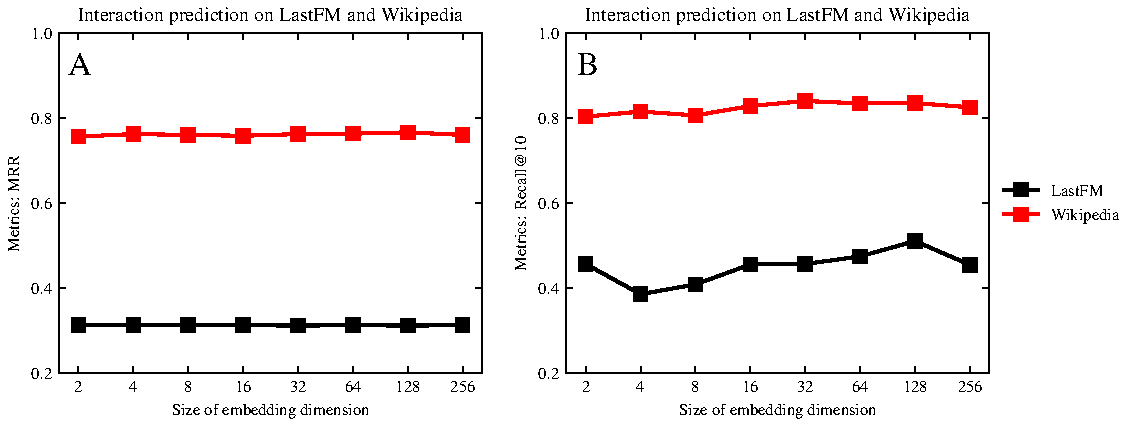
\includegraphics[width = \textwidth]{image/lastFM-wiki.pdf}
    \caption{Robustness of JODIE replication}
    \label{emb-size}
\end{figure}

\subsection{Additional result}
We decided to extend our analysis by testing the impact of the \texttt{split} (see Section \nameref{sec:trainning}) on the performance of the JODIE model. As a reminder, the original study doesn't consider \texttt{split} as a hyper-parameter but as a constant fixed to 500. 
Figure ~\ref{split} illustrates the significant impact of this parameter on the overall results. Regardless of the embedding size, as the value of \texttt{split} increases, so does the performance. By augmenting the \texttt{split} value from 5 to 500, the performance increases by 0.14 in AUC for the different embedding sizes. Then, scaling up from 500 to 50000, the performance increases by a further 0.08. We can explain this gain by the fact that the model performs back-propagation after each time step defined by \texttt{split}. Thus, by increasing the number of \texttt{split}, we increase the number of back-propagations. This result suggests that higher values of \texttt{split} may improve the performance, but its choice must be made by considering the execution time and complexity, which increase significantly with larger \texttt{split}.

\begin{figure}[htbp]
    \centering
    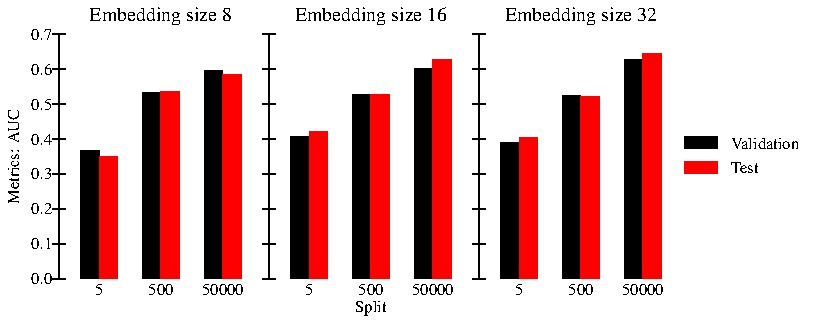
\includegraphics[width = \textwidth]{image/split.pdf}
    \caption{Comparison the robustness of the JODIE model as a function of the hyper-parameter \texttt{split}.}
    \label{split}
\end{figure}

\section{Conclusion}
We successfully replicated the original code provided by the authors and reproduced their results. Even though our replication more or less matches the results, we found some slight differences compared to them. This can be explained by a variation due to the initialization. However, for the LastFM dataset, our reproduction results clearly outperform those claimed in the original study. We suspect some reporting errors in the paper. We have also shown that the embedding size slightly impacts the result if a different evaluation metric than the one proposed in the original article is used. This fact mitigates the author's claim that the embedding size has no impact on the overall performance of their model. Finally, we have found that the split parameter strongly affects the overall performance. This hyper-parameter, unexplored in the original paper, must be tuned according to a complexity-performance trade-off of the model. As a perspective, we think it would be beneficial to use the focal loss~\cite{https://doi.org/10.48550/arxiv.1708.02002} instead of the standard cross entropy loss in the JODIE model to alleviate the issue we have met with unbalanced classes.